\chapter{Experimental Setup}
\label{chap:experiment}
In this chapter the setup as well as the methods by which the C. sphaerospermum samples are prepared and treated are described. All experiments were conducted in the laboratory of the group for plasma physics at the Kyoto Institute of Technology led by Assoc. Prof. Kazou Takahashi. The work was done in collaboration with Shinano Kinoshita and based on previous research \cite{kit} conducted by Tomoya Ohara and her.

\section{APP Setup}
To create an atmospheric plasma a DBD is used. The setup consists of two pairs of isolated electrodes. The electrodes are separated by a dielectric material which prevents a continuous discharge. A diagram of entire setup is shown in figure \ref{fig:setup} and a photograph of its implementation is shown in figure \ref{fig:photo}. The experiment is contained with a transparent box to prevent contamination and control the atmosphere around the plasma and mould. Through a tube dry or mist, generated by an ultrasonic mist generator, can be introduced into the chamber. While the effect of humidity has been studied in the past \cite{kit} it is not the focus of this work. Therefore, the mist generator is not used in experiments.
\begin{figure}
    \centering
    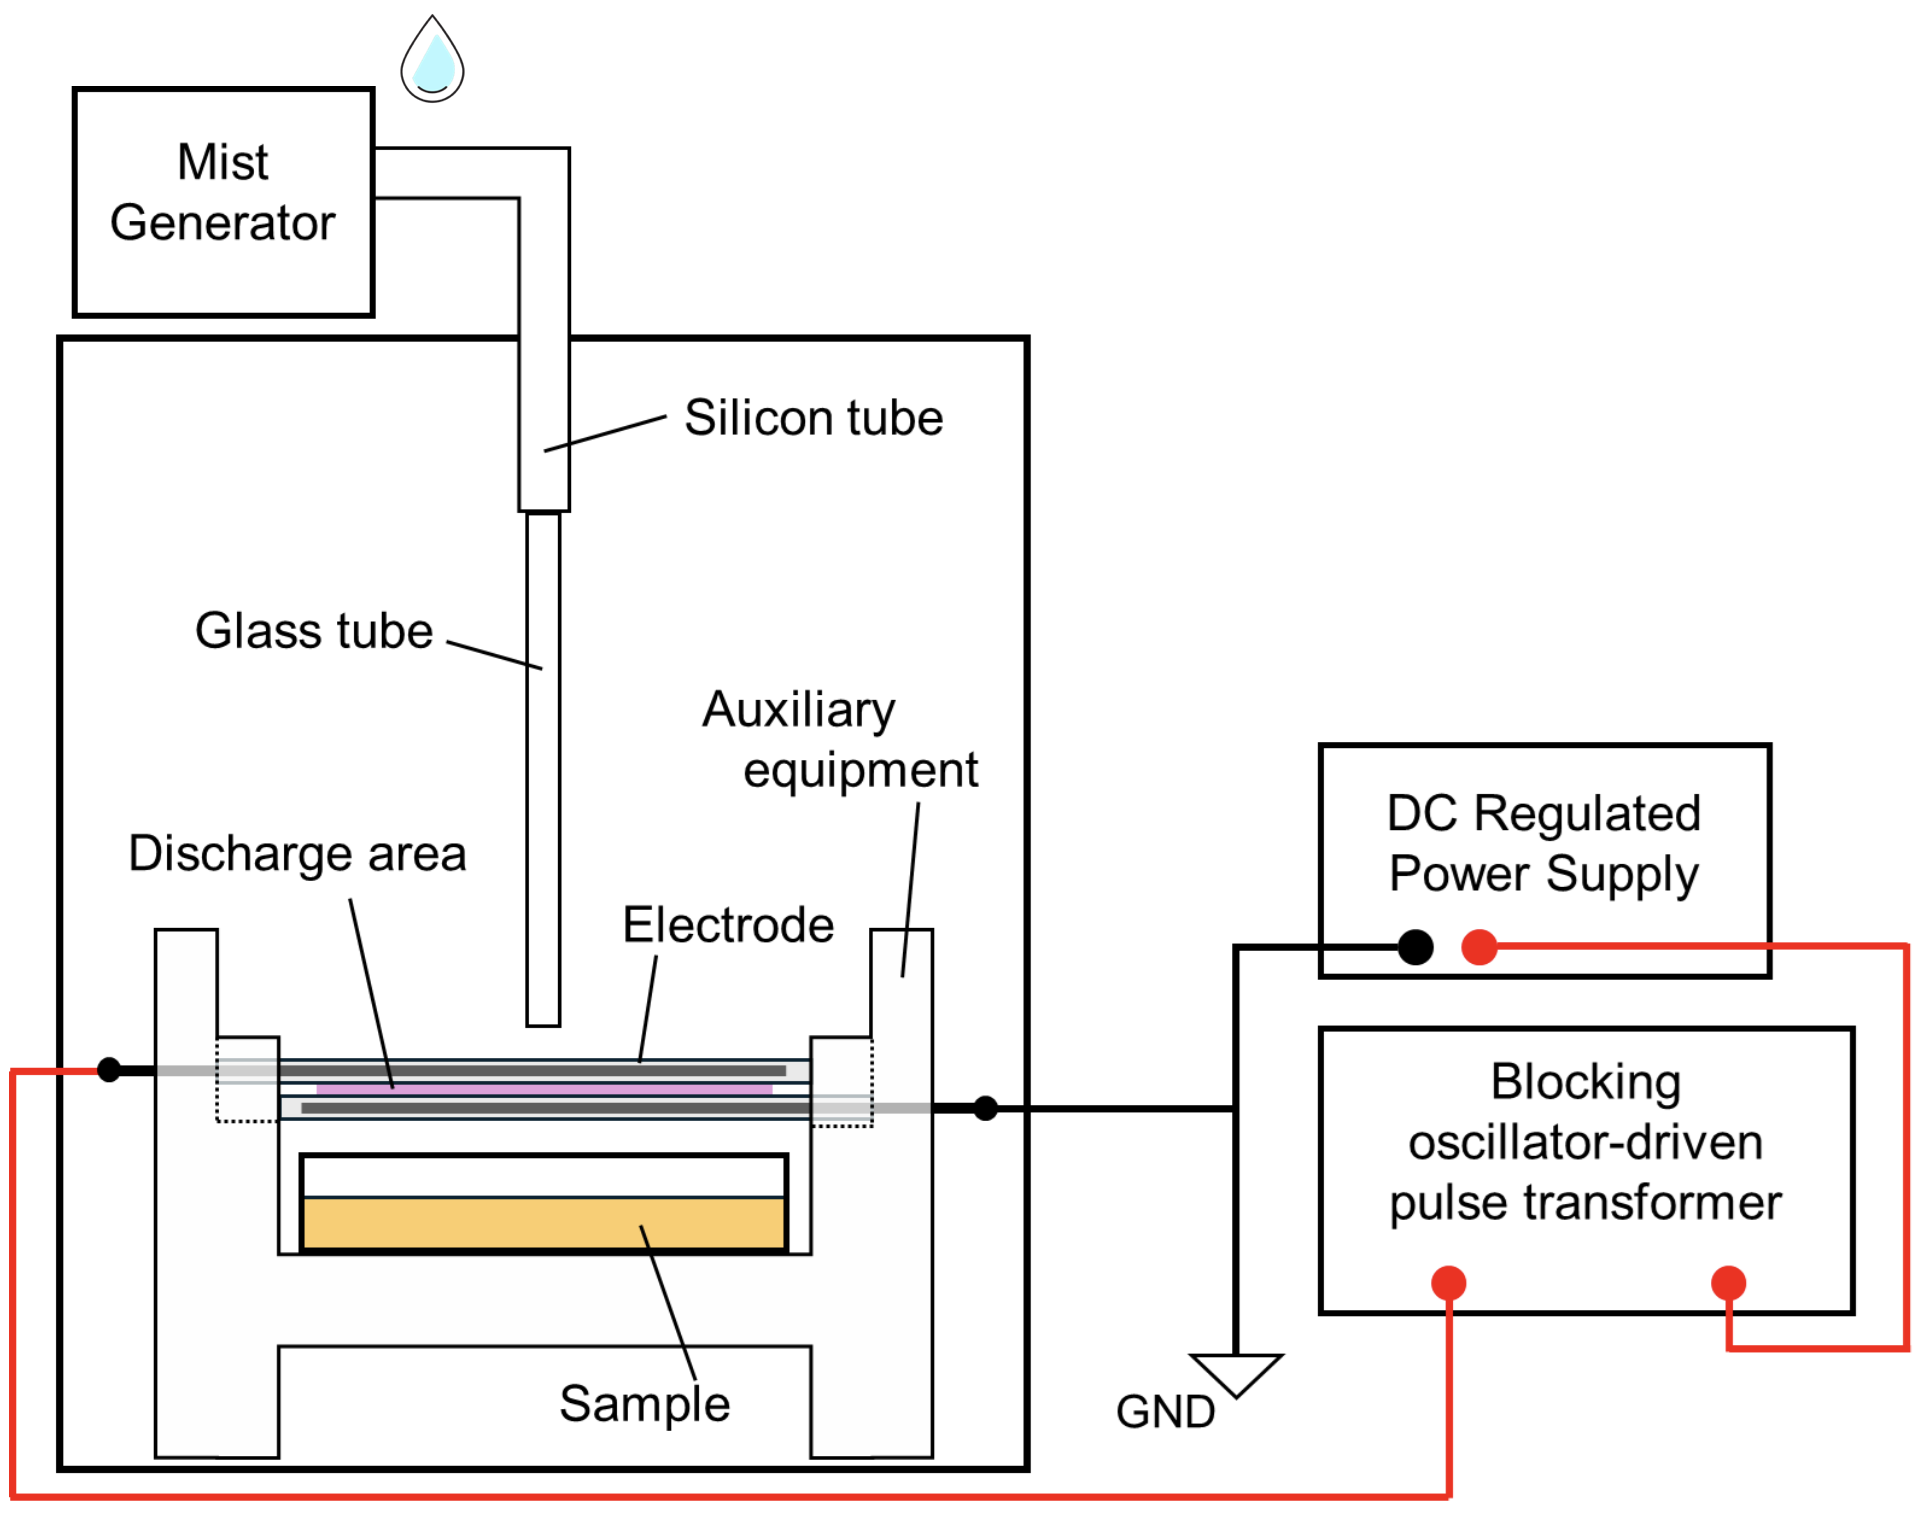
\includegraphics[width=.6\textwidth]{images/Process_setup.png}
    \caption[Diagram of the setup]{This figure shows the experimental setup. The APP is generated between two pairs of electrodes. The entire setup is placed in a box to prevent contamination. The sample is placed underneath the discharge area. A tube can provide water mist and dry air to control the humidity in the chamber. A power supply and a blocking oscillator provide an oscillating voltage to the electrodes.}
    \label{fig:setup}
\end{figure}

\begin{figure}
    \centering
    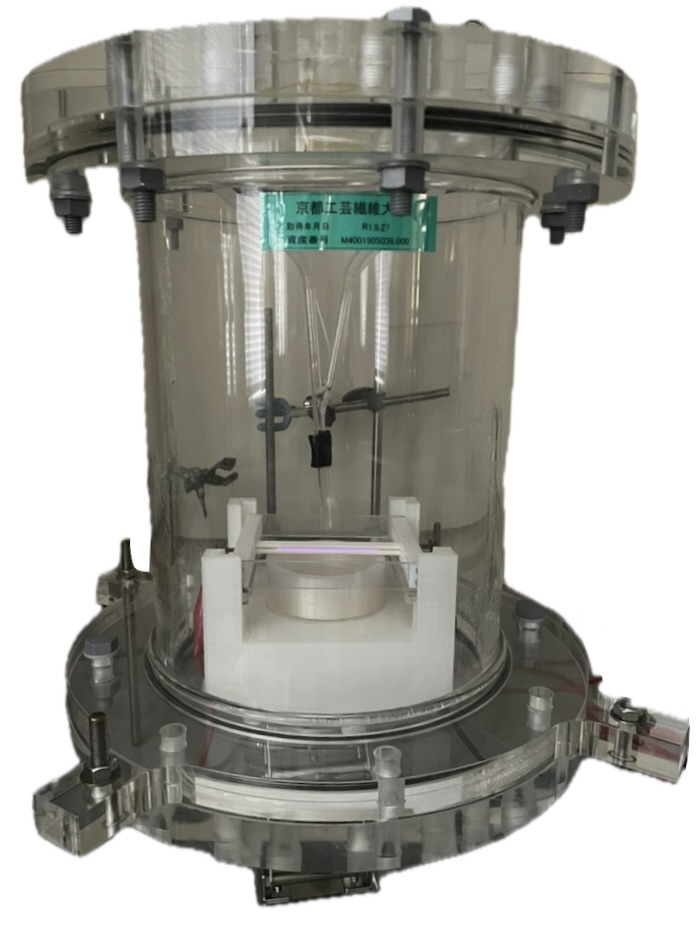
\includegraphics[width=.5\textwidth]{images/Setup_photo.jpeg}
    \caption[Photograph of the setup]{Photograph of the experimental setup.}
    \label{fig:photo}
\end{figure}

\subsection{Dielectric Barrier Discharge}
\label{sec:dbd}
For the discharge four electrodes are used. They are coated in ceramics. Figures \ref{fig:dbd} and \ref{fig:plasma} show the exact discharge setup. The DBD is powered by a high voltage DC power supply that is then converted to an AC voltage with a blocking oscillator. An oscilloscope is used to measure the voltage and current of the discharge. Figure \ref{fig:signal} shows the voltage and current signal of the DBD. The discharge area has a small volume and radiation is only emitted between the electrodes. 
\begin{figure}
    \centering
    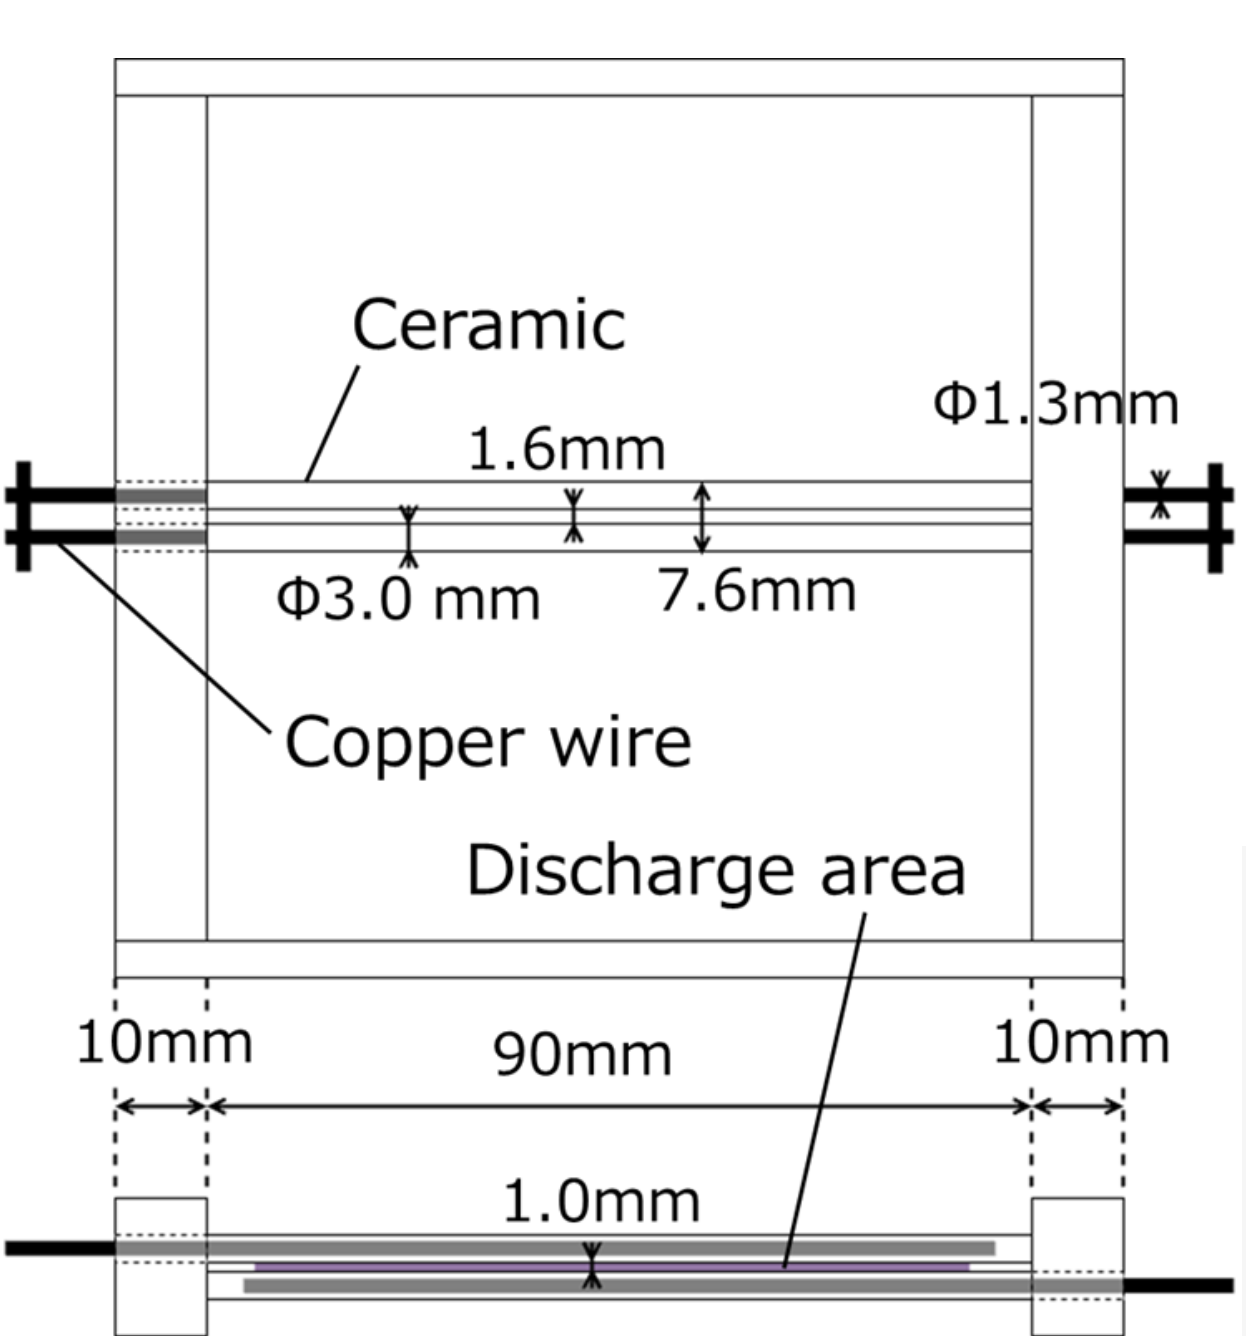
\includegraphics[width=.65\textwidth]{images/APP_setup.png}
    \caption[Technical sketch of the DBD setup]{Technical sketch of the DBD setup. On the top the view from above the DBD setup is shown, on the bottom the side view. The APP is generated by a DBD with a frequency of 13.56 MHz and a voltage of 13 kV. This diagram has kindly been provided by Shinano Kinoshita.}
    \label{fig:dbd}
\end{figure}

\begin{figure}
    \centering
    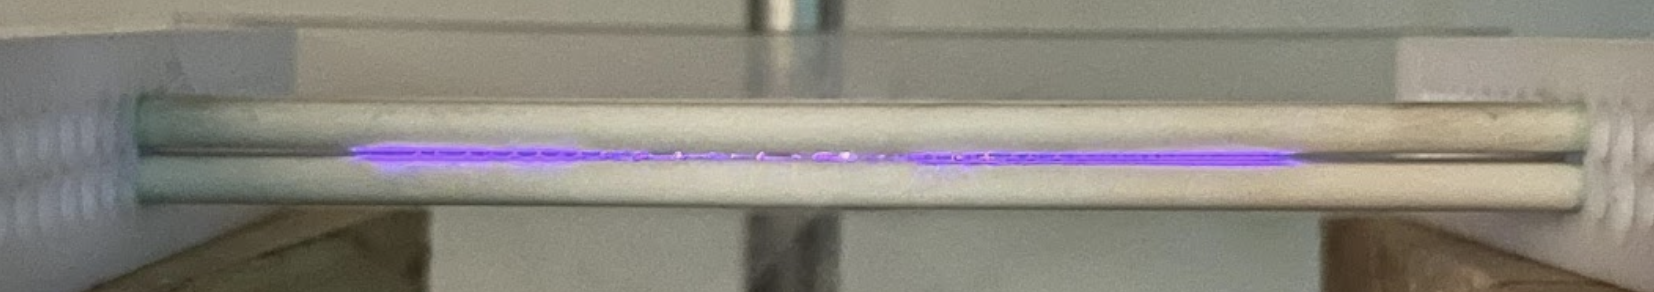
\includegraphics[width=1\textwidth]{images/Plasma.png}
    \caption[Image of the APP]{Image of an ignited plasma at atmospheric pressure between the electrodes.}
    \label{fig:plasma}
\end{figure}


\subsection{Measurement of the Plasma Spectrum}
\label{sec:oes}
To measure the optical spectrum of the plasma a photonic multichannel analyser, the \textsc{PMA-12} by Hamamatsu, is used. It is able to measure spectra down to 200 nm and up to 1200 nm. The spectrometer is connected to a computer via USB and the data is recorded with a software that can automatically correct for its spectral response. Figure \ref{fig:oes} shows a spectrum of the plasma recorded with the spectrometer. It is later analysed in section \ref{sec:oes_analysis}.  

\begin{figure}
    \centering
    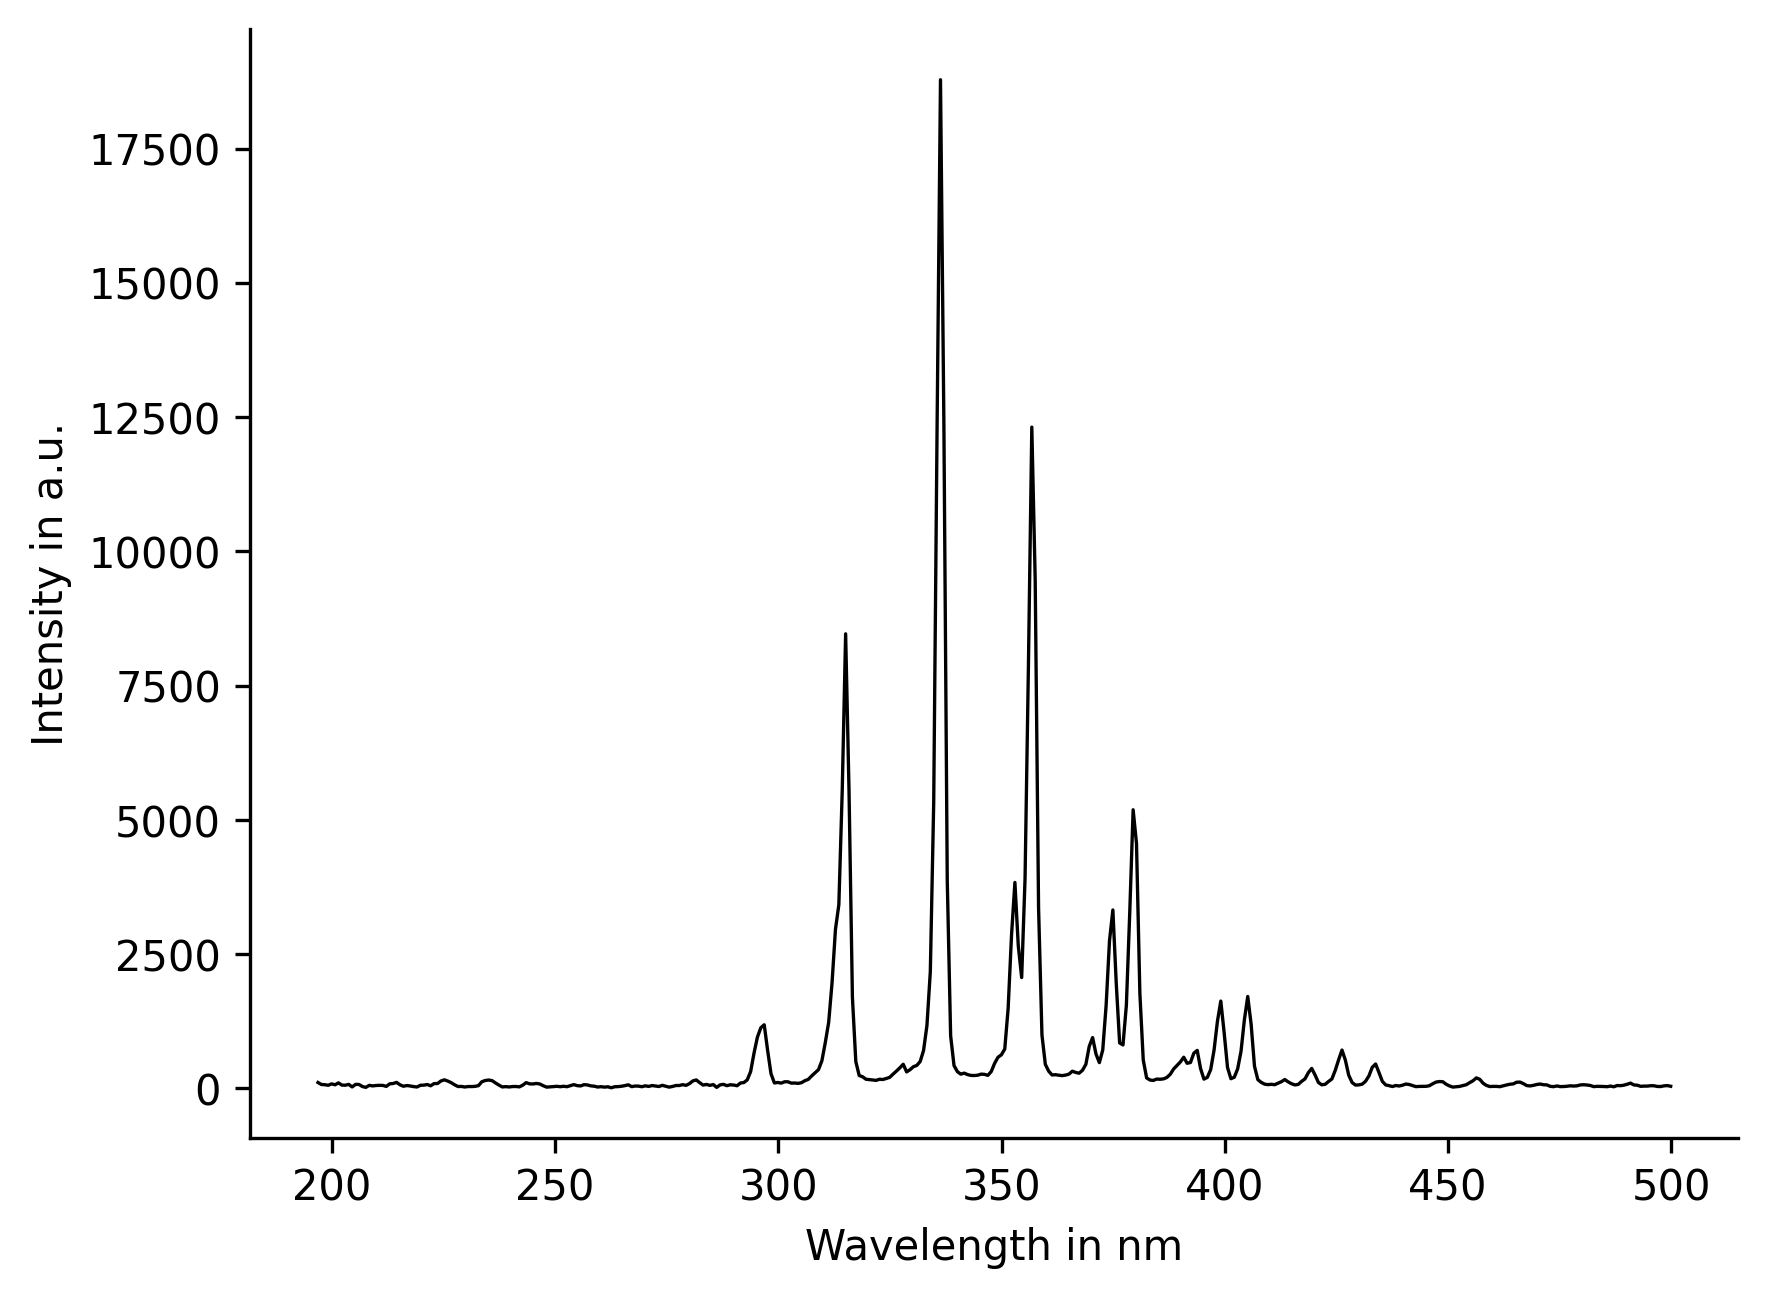
\includegraphics[width=.8\textwidth]{images/OES.png}
    \caption[Raw OES spectrum of the APP]{Raw OES spectrum of the plasma at atmospheric pressure with ambient air as the working gas. The peaks are anlysed in section \ref{sec:oes_analysis}.}
    \label{fig:oes}
\end{figure}

\section{Preparation of Samples}
The samples are grown in Petri dishes on an agar medium. The medium is prepared in the lab beforehand. Table \ref{tab:medium} shows its composition. To create new samples spores of the fungus C. sphaerospermum are collected from thriving colonies. They are dissolved in sterilized water and then scraped off the surface by using a cotton swab. The solution containing the spores is then diluted in two or three steps of 1:10 to reach a concentration of around $3.5\times 10^4$ or $3.5\times 10^3$ spores per ml. This is then verified using a cell counting plate under a microscope. 100 \textmu l of the diluted solution are then spread on fresh agar media and are ready for treatment.

After treating the spores with plasma, UV or none the samples are incubated in an incubator for multiple days at their ideal growing temperature of 25 °C. When the incubation period is over the samples are taken out and the number of colonies is counted to get an estimate of the inactivation percentile. Each experiment contains at least two control samples that are not treated and can be used as a reference.

\begin{figure}
    \centering
    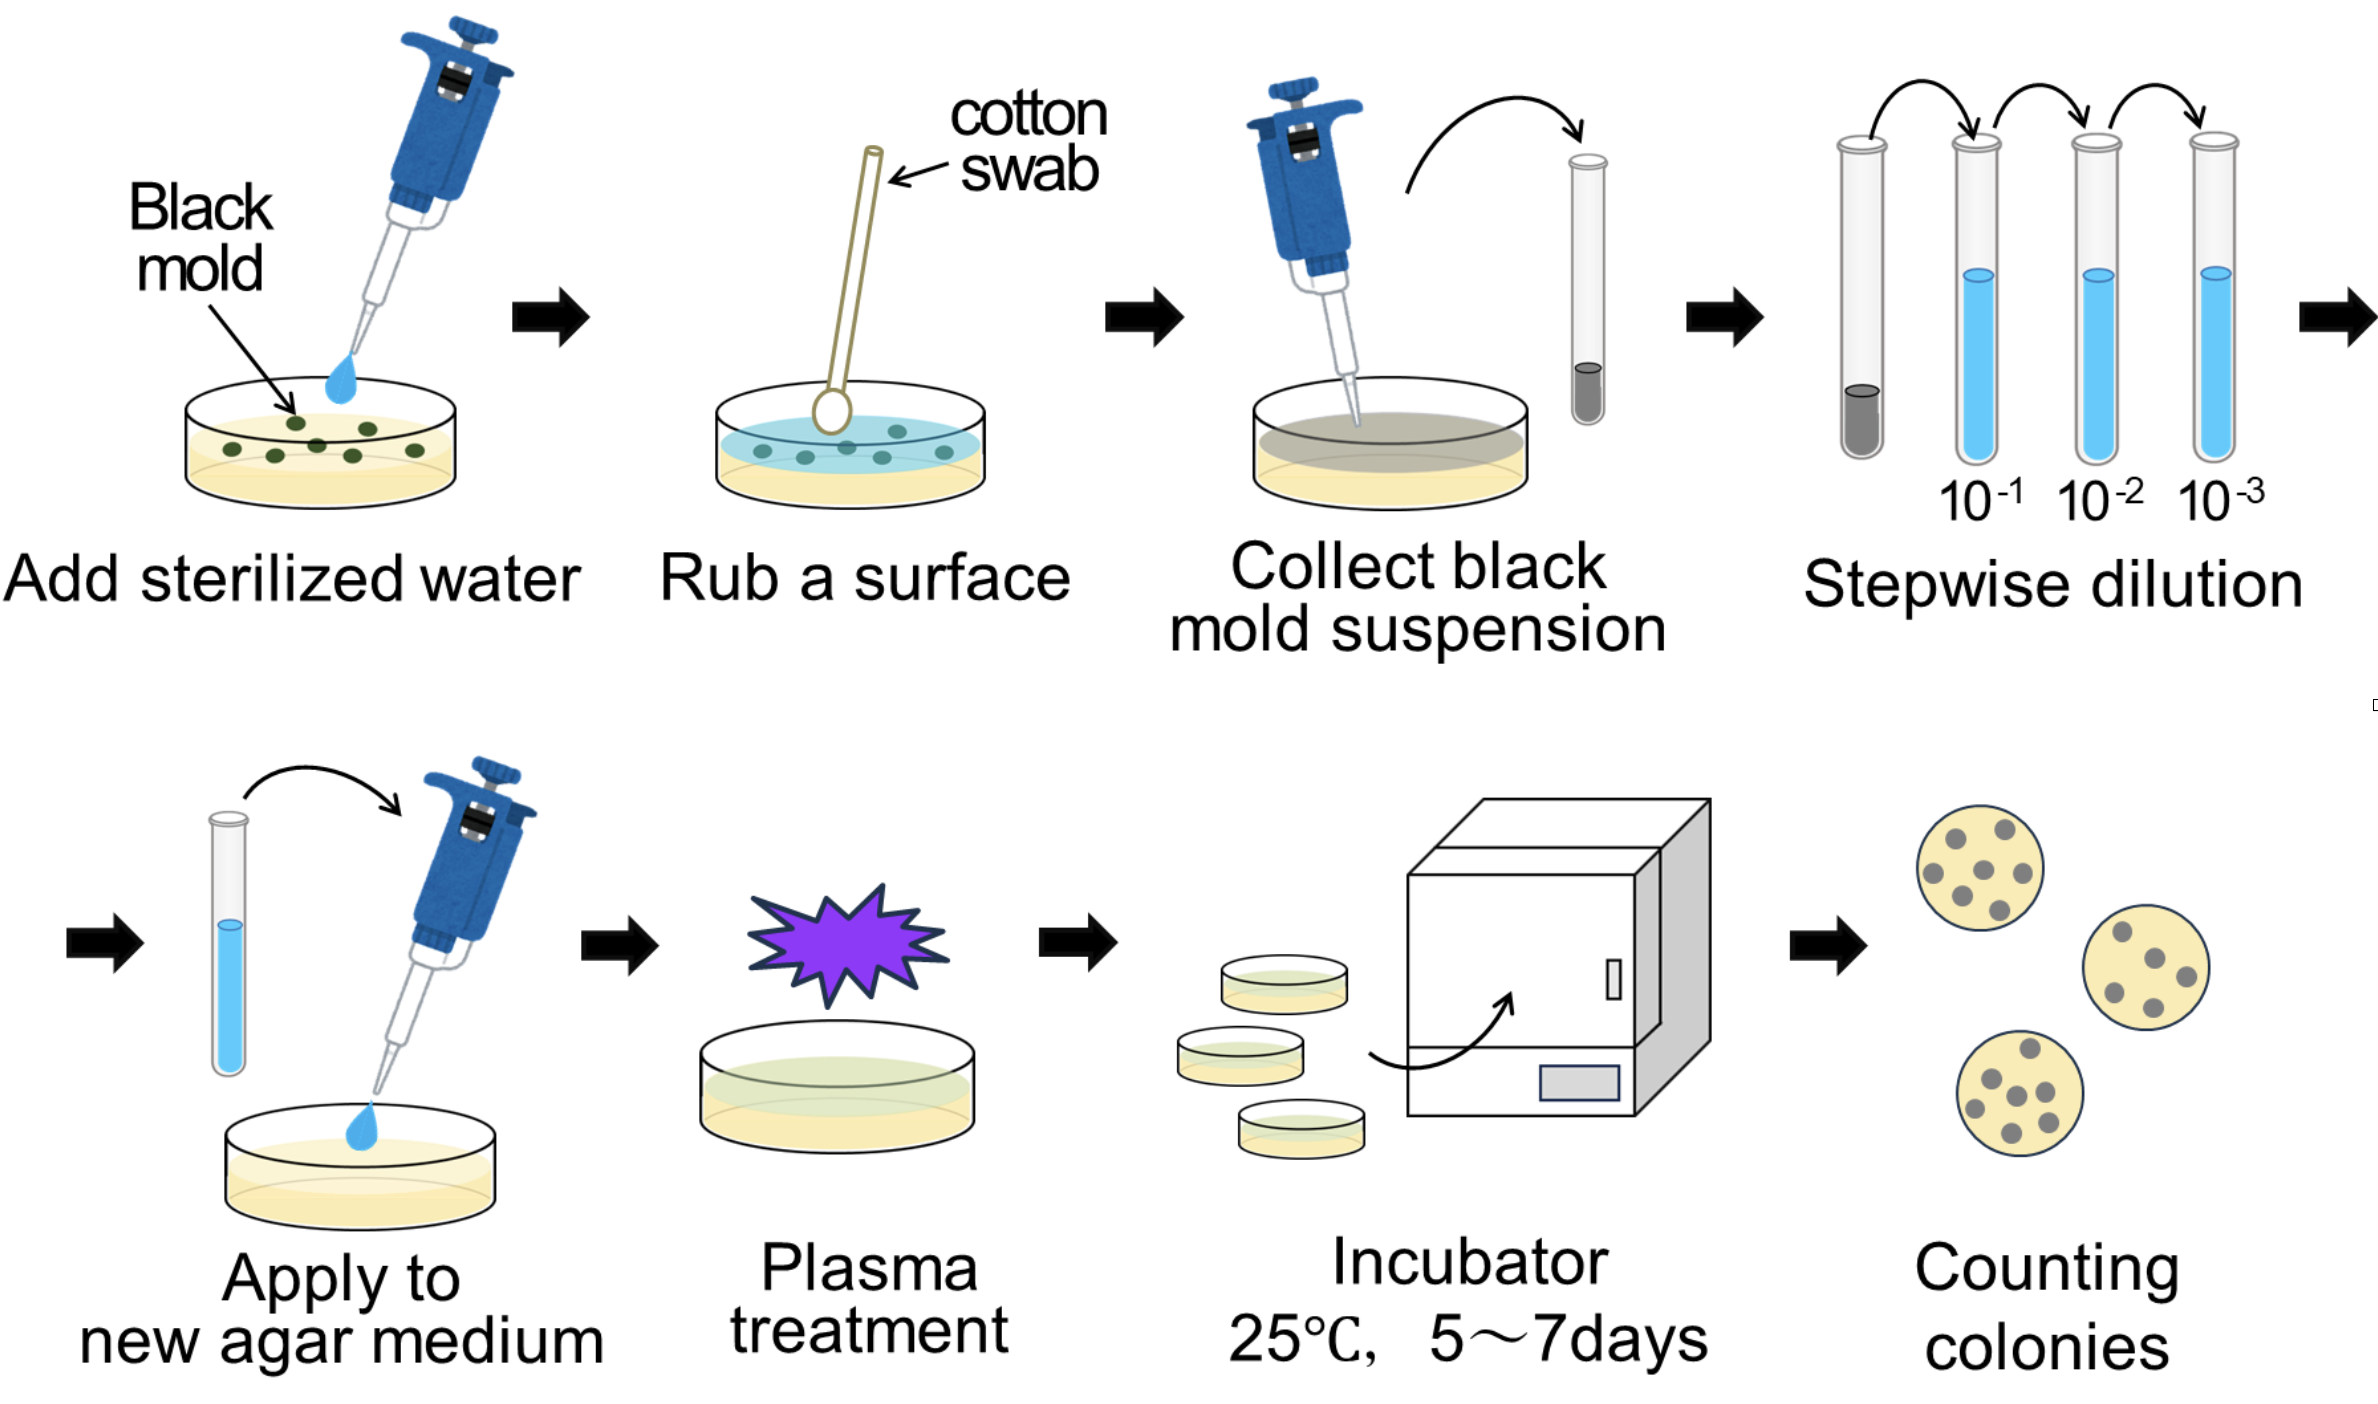
\includegraphics[width=1\textwidth]{images/Process.png}
    \caption[Diagram of the experiment process]{Diagram of the experiment process and the preparation of samples. The fungus is cultivated on an agar medium and stored in Petri dishes. Spores are collected by dissolving them in sterilized water and then their concentration is diluted in steps to the desired concentration. The samples are then treated with the APP and the inactivation rate is measured by counting the colonies on the agar medium.}
    \label{fig:process}
\end{figure}

\section{UV Exposure}
To test the effects of UV radiation on the samples before exposing them to the radiation emitted by the plasma, a UV lamp is used. The lamp is inside a clean bench to allow exposure to the UV light while preventing contamination. Figure \ref{fig:uv} shows the spectrum of the UV lamp. It emits light in the range of 200 nm to 450 nm with its main peak at 254 nm. The data sheet\footnote{The lamp used is the sterilization lamp \textsc{GL15} by Toshiba} of the lamp states that it emits radiation with an irradiance of 51 \textmu W/cm\textsuperscript{2}. This is measured at the radius of the cylindrical glass tube that encloses the lamp. To estimate the dose of radiation that the samples are exposed to, the effective irradiance $I_\text{eff}$ at a given distance from the lamp must first be determined. For this, the distance $r$ from the lamp to the sample is measured, and the irradiance is calculated using the formula:

\begin{equation}
I_\text{eff} = I_0 \cdot \frac{r_0}{r},
\end{equation}

where $I_0$ is the irradiance at the radius $r_0$ of the lamp. Here it is assumed that the lamp acts more like a thin line source of light than a point source, which only applies for short distances from the lamp. Once the effective irradiance is known, the dose $D_\text{UV}$ can be calculated as:

\begin{equation}
D_\text{UV} = I_\text{eff} \cdot t,
\label{eq:uv_dose}
\end{equation}

where $t$ is the time of exposure. This provides an estimate of the UV dose received by the samples during irradiation. In the setup used for the experiments the effective irradiance computes to 1.14 \textmu W/cm\textsuperscript{2} at a distance of 58 cm from the lamp.


\begin{figure}
    \centering
    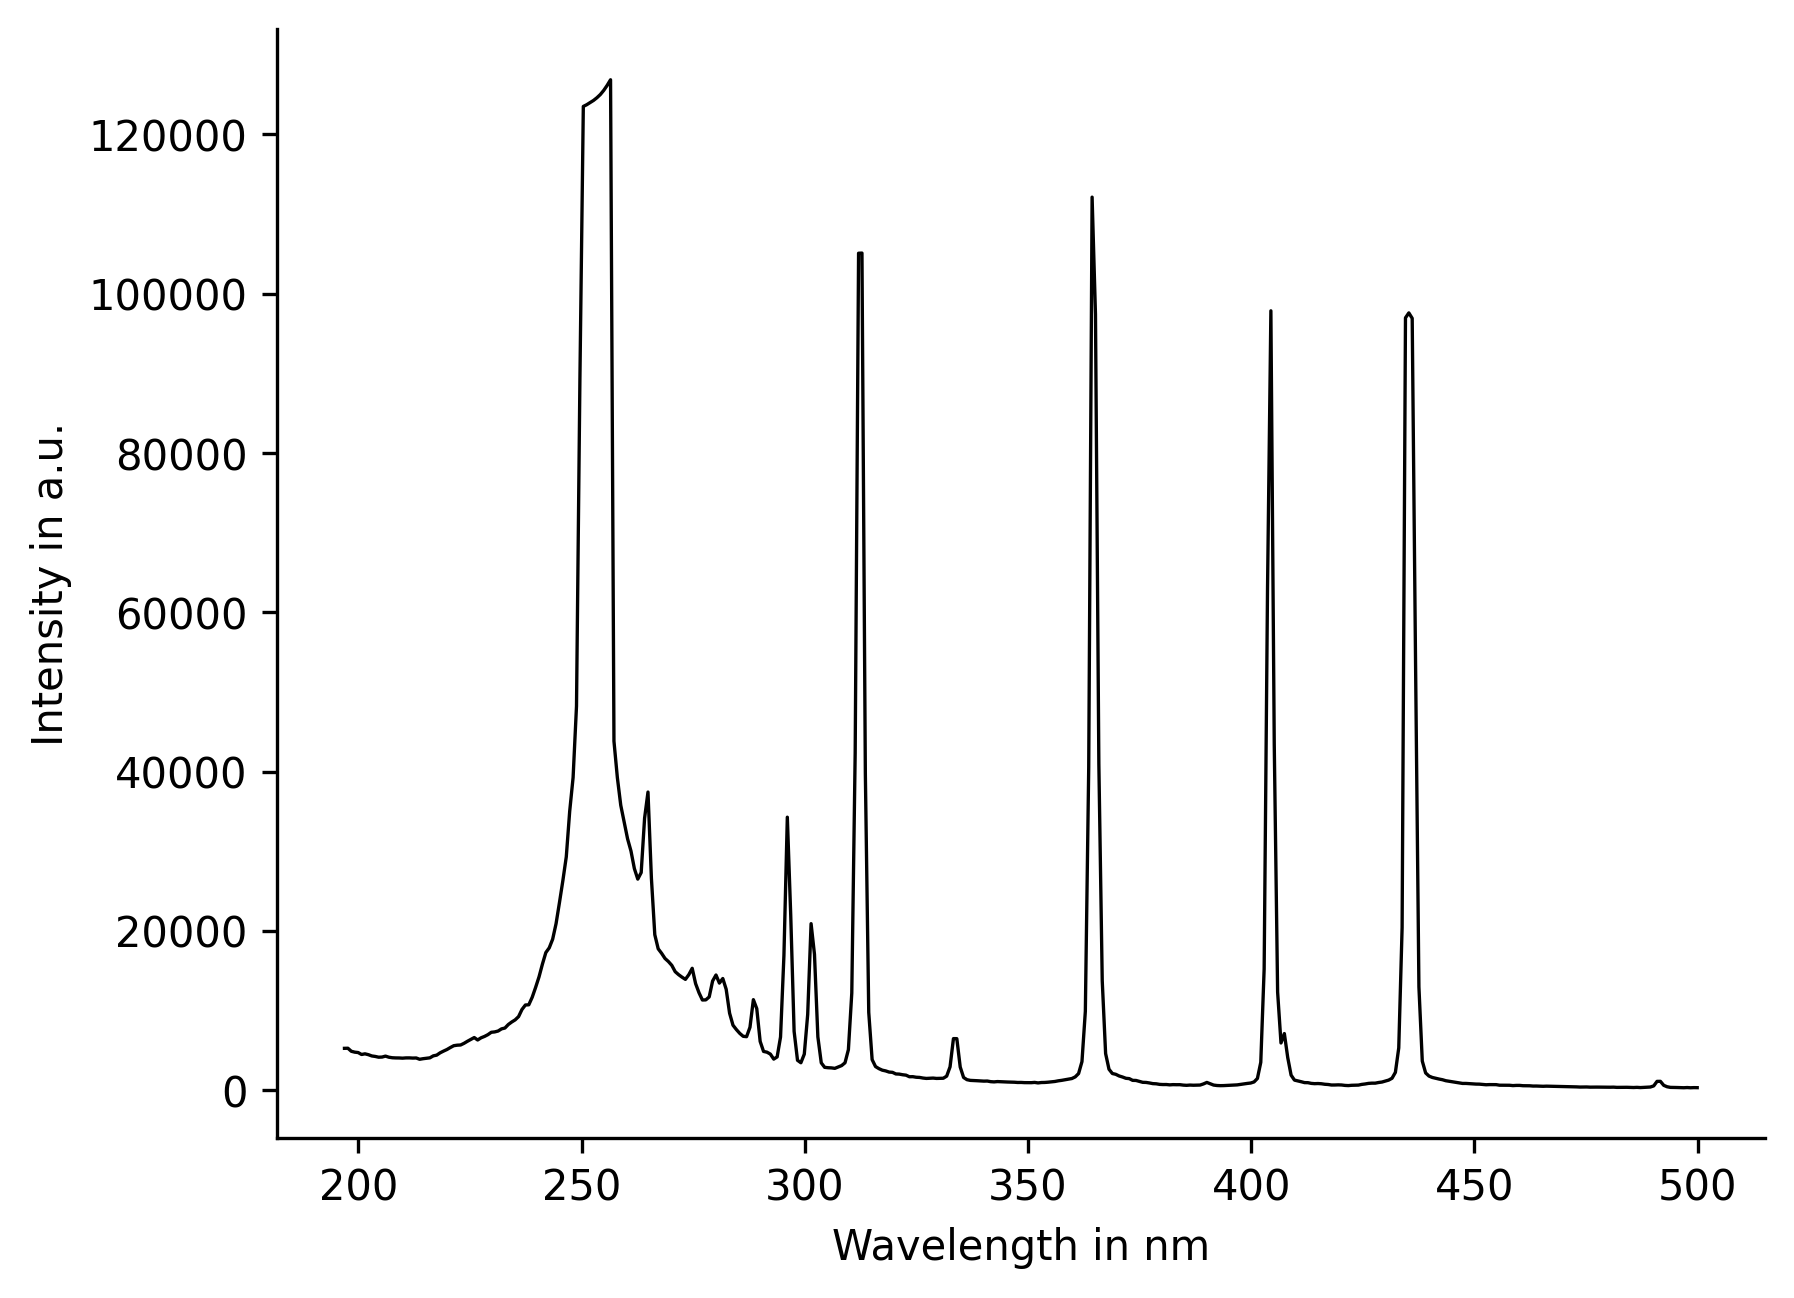
\includegraphics[width=.8\textwidth]{images/UV_lamp_no_glass.png}
    \caption[Spectrum of UV lamp]{Spectrum of the UV lamp. The main peak is at 254 nm. The spectrum was measured with the same spectrometer from section \ref{sec:oes}.}
    \label{fig:uv}
\end{figure}

\section{Plasma Treatment}

\subsection{Full Plasma Treatment}

\subsection{Isolation of Radiation}
To isolate the effects of the radiation emitted by the plasma from the reactive chemicals a transparent barrier is used. The barrier is made of quartz glass and is also transparent to visible light. It is 8 mm thick. To hold the barrier in place a mount is designed and 3D printed from PLA. The mount is designed to hold the barrier in place and to allow for easy removal.

To verify the transparency of the quartz glass, the spectrum of the UV lamp shown in Figure \ref{fig:uv} is measured with and without the barrier. The results are found to be nearly identical in the range that is relevant for this experiment, so no correction is needed. 


